\subsection{In-depth electromagnetic simulation}

To get an idea of how the design will behave in real life, a more thorough simulation is necessary.
Figure \ref{fig:big-sim} shows the test setup in \emph{ADS Momentum}.

\begin{figure}[h t b p]
	\centering
	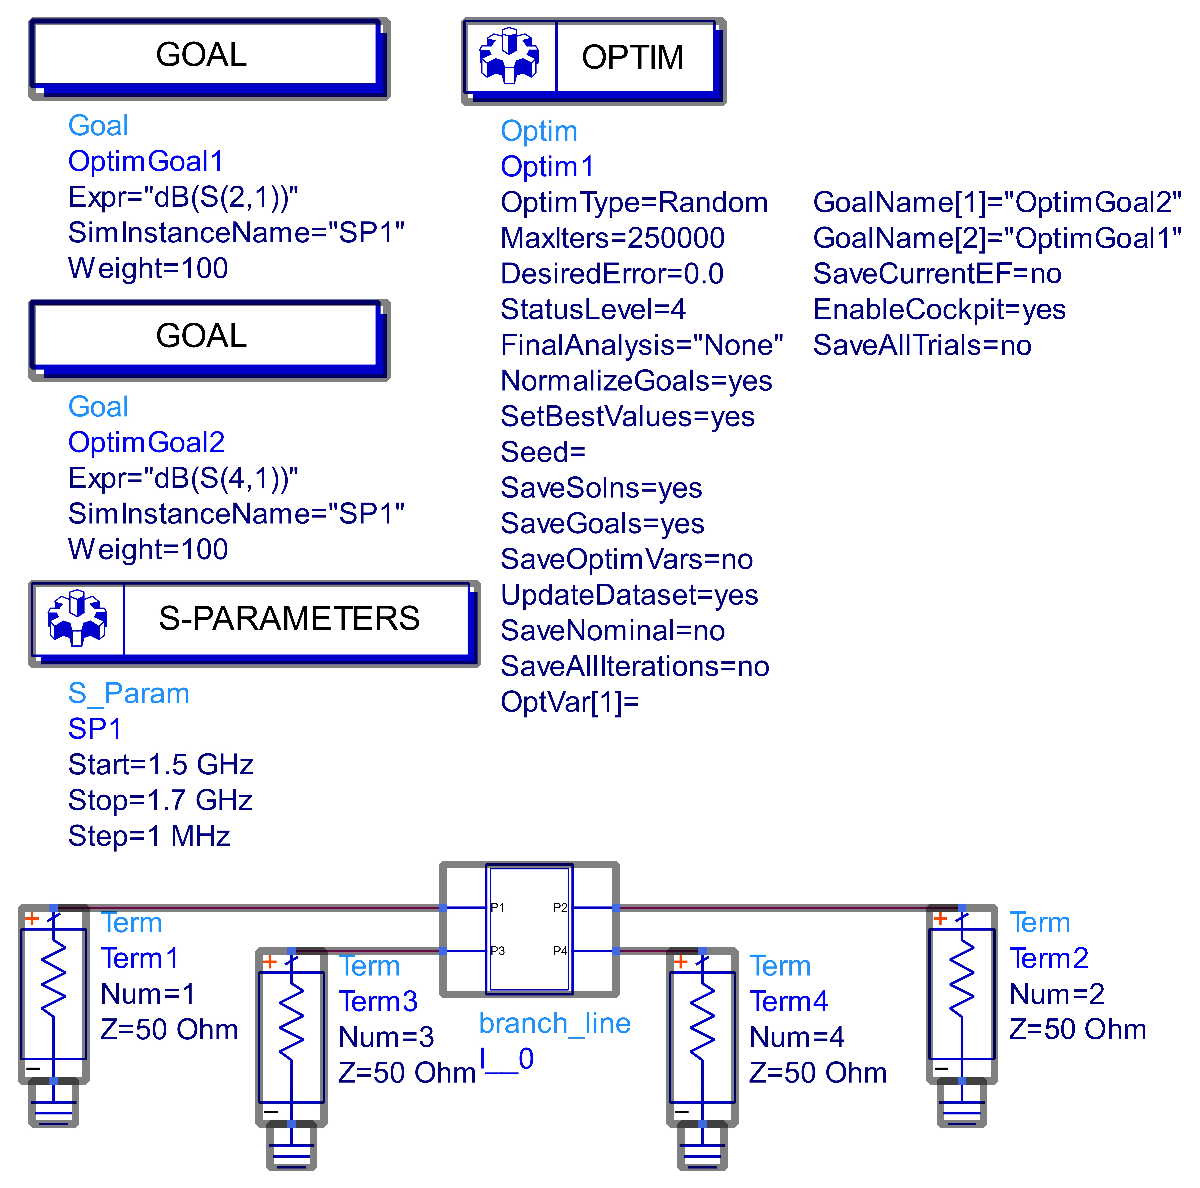
\includegraphics[width=\textwidth,keepaspectratio]{figures/big_sim_sch.eps}
	\caption{Simulation schematic in ADS.}
	\label{fig:big-sim}
\end{figure}

Running this simulation with optimization, we obtain a new geometry for the MS-BLDC.
These values are exempt from this paper, but we note that they were very similar yet different from the initial values. \par

Figures \ref{fig:big-sim-41-21} and \ref{fig:big-sim-phase} shows how this new, optimized geometry affects S(2,1) and S(4,1).
Figure \ref{fig:big-sim-field-colors} show the intensity of current in the MS-BLDC.

\begin{figure}[h t b p]
	\centering
	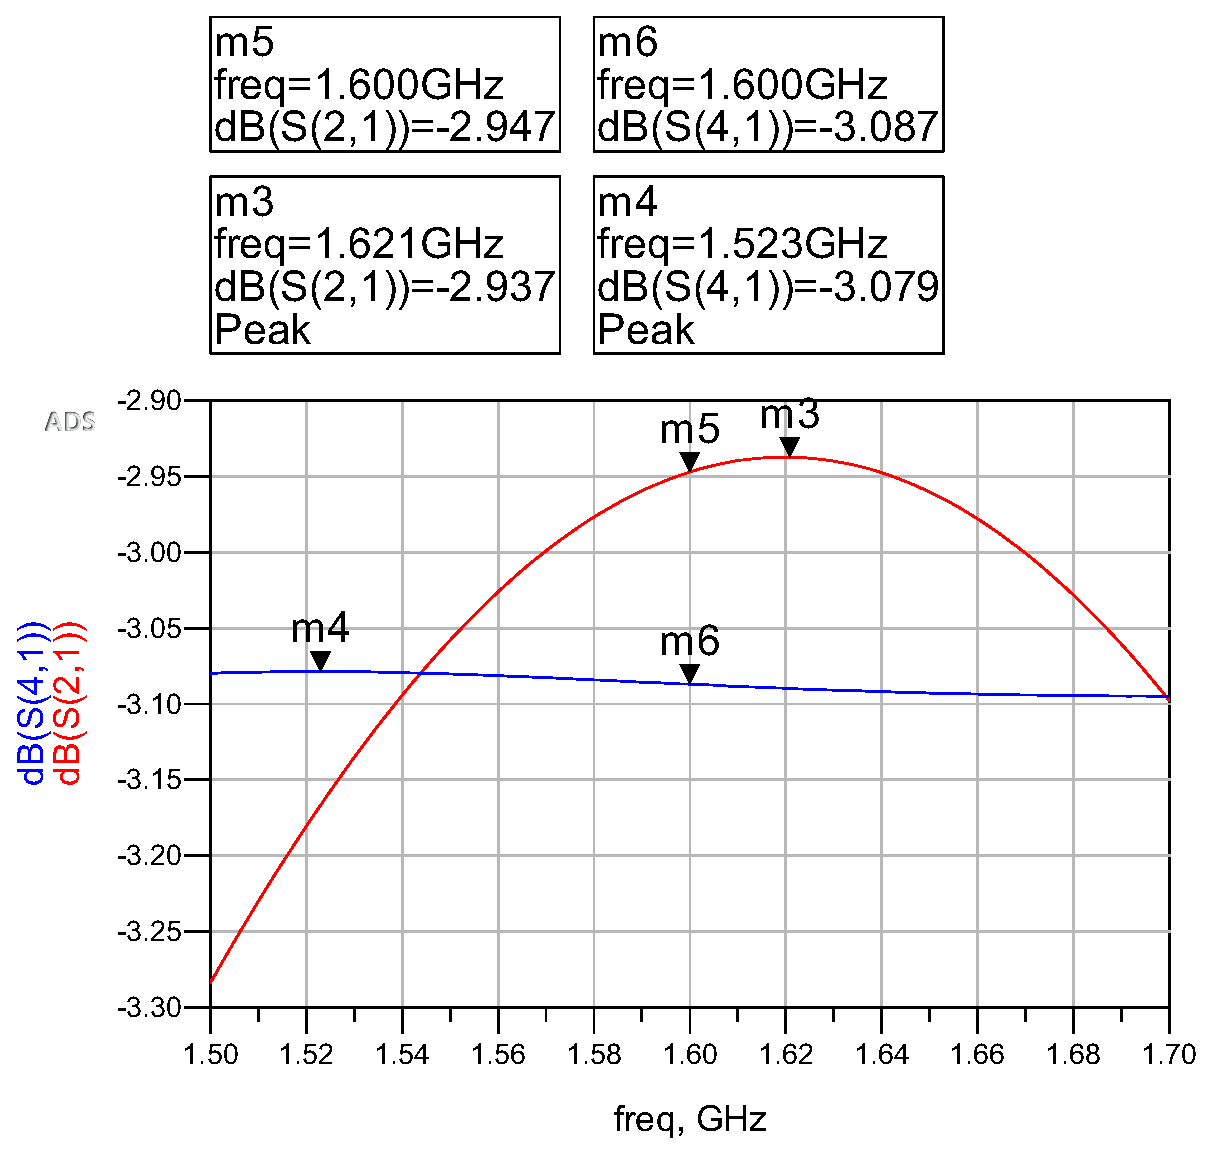
\includegraphics[width=\textwidth,keepaspectratio]{figures/big_sim_41_21.eps}
	\caption{Simulated S(2,1) and S(4,1) with new geometry.}
	\label{fig:big-sim-41-21}
\end{figure}

\begin{figure}[h t b p]
	\centering
	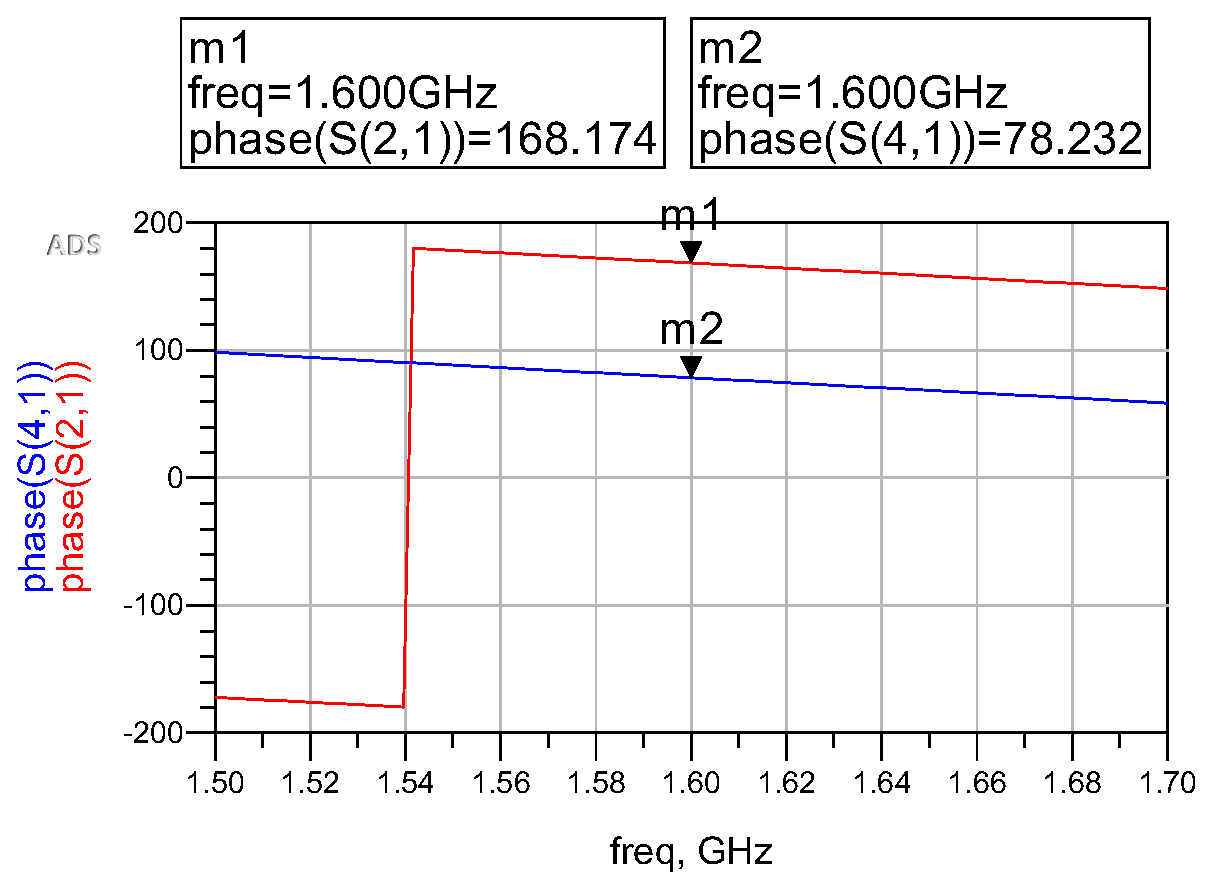
\includegraphics[width=\textwidth,keepaspectratio]{figures/big_sim_phase.eps}
	\caption{Simulated S(2,1) and S(4,1) phase difference with new geometry.}
	\label{fig:big-sim-phase}
\end{figure}

\begin{figure}[h t b p]
	\centering
	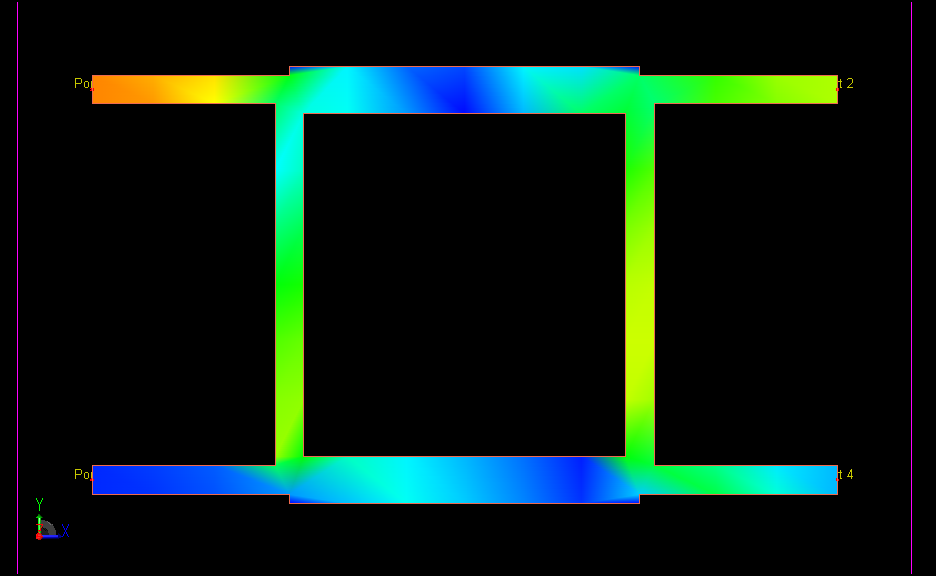
\includegraphics[width=\textwidth,keepaspectratio]{figures/sim_field_colors.png}
	\caption{Simulated current intensity in MS-BLDC.}
	\label{fig:big-sim-field-colors}
\end{figure}